\documentclass{article}

%%%%%%%%%%%%%%%%%%%%%%%%%%%%%%%%%%%%%%%%%%%%%%%%%%%%%%%%%%%%%%%%%%%%%%%

\usepackage{url}
\usepackage{graphicx}
%\usepackage{fullpage}

% Remove red border around refs and make them stand out.
\usepackage[colorlinks=true,linkcolor=blue]{hyperref}

%%%%%%%%%%%%%%%%%%%%%%%%%%%%%%%%%%%%%%%%%%%%%%%%%%%%%%%%%%%%%%%%%%%%%%%
%% Check these macro values for appropriateness for your own document.

\title{IS3 Group Report}

%%authors
\author{
  Richard Fleming \\
  James Gallagher \\
  Craig McLaughlin \\
  Victor Pantazi \\
  Gordon Reid \\
  Ross Taylor}

%%release date 
\date{\today}

%%%%%%%%%%%%%%%%%%%%%%%%%%%%%%%%%%%%%%%%%%%%%%%%%%%%%%%%%%%%%%%%%%%%%%%

\begin{document}

%%%%%%%%%%%%%%%%%%%%%%%%%%%%%%%%%%%%%%%%%%%%%%%%%%%%%%%%%%%%%%%%%%%%%%%

\maketitle

%%%%%%%%%%%%%%%%%%%%%%%%%%%%%%%%%%%%%%%%%%%%%%%%%%%%%%%%%%%%%%%%%%%%%%%
%% Standard section for all documents

\section{Preamble}

In this report, various popular calendars are evaluated using the
Think-aloud evaluation technique to identify desirable features of a
modern calendar. Three paper prototypes are designed by pairs from the
team, and based on these paper prototypes, a final paper prototype will
be detailed.


\begin{itemize}
\item Give an overview of your paper prototypes, the early designs and
how you came to your final prototype design;

\item Explain how they work;

\item Report on your heuristic evaluation/think aloud, any problems you
found and how you resolved them (include the key paper prototypes that
you built);
\end{itemize}

\section{Overview}

Our prototypes were based on the Facebook, OS X, Evolution on Scientific
Linux, 30 Boxes, and Google calendars. For prototyping and evaluating we split up
into two person teams. For the purposes of the discussion the teams are
labelled based on the calendars they evaluated.

The final paper prototype was a combination of our findings from the
calendars.

\section{Calendar on OS X}

Apple Inc.'s use of skeuomorphism creates an interface similar to a real 
calendar with simulated page rips, faux-leather textures for UI
elements, and page turn animations. The design of the paper prototype
based on this calendar borrowed from the ethos of Apple's design.

\subsection{Think-aloud Evaluation}
The participant was asked to perform a series of set tasks, incorporated
into a scenario. Below the tasks are described and feedback from the
participant noted:

\begin{itemize}
\item Add an event for a friends party.

There was an intuitive plus button on the top-left of the window, which
opened a dialog box for adding an event on the currently selected day.

\item Change the event to the following week.

\item Delete the event.

\item Set a recurring event.

\item Find out which days of the month are the busiest and quietest
respectively

The year view for the calendar fills days in colour indicating the
number of appointments scheduled for that day, in a spectrum from
red (busy) to white (quiet). This made this particular task incredibly
simple and it is this reason this feature was included in an early
paper prototype (see Section~\ref{sec:osxpp}).

\item Change the calendar categories currently displayed.
\end{itemize}

The participant noted feeling uncomfortable during the evaluation as it
was unnatural for the them to have to vocalise their actions. At some
points during the experiment, the participant seemed confused or
surprised by the feedback from the system, occasionally expressing
uncertainty on how to proceed further with the task.

\subsection{Paper prototype}
\label{sec:osxpp}

The paper prototype has a minimalist design with three views: week,
month, and year. These views are available through three buttons that
are always on the screen at the top centre-right. The currently selected
view is coloured differently than the others and appears depressed.

The initial draft of the event dialog pop up window, that would be
shown when a user decides to add a new event, or wishes to edit or
delete an existing event, is illustrated in Figure~\ref{fig:addevent}.

A user is able to have multiple calendars, perhaps to split up work and
home events. This screen (Figure~\ref{fig:viewcal}) allows a user to
choose which calendars to view, add a new calendar, or delete an old
calendar and associated events.

The month view for our calendar is shown in Figure~\ref{fig:monthview}.
This view is also the default view. Events are listed in summary form
in the grid of squares. When a user clicks on the grid, the full listing
for the selected day is shown in the side panel on the right.

The year view for our calendar is depicted in Figure~\ref{fig:yearview}.
The primary purpose of the view is to allow daily summaries to be
visualised. Similar to Apple's Calendar application, days which are
busy are coloured in an increasing level of opaqueness, dependant on
the number of events added for the associated day.

\section{Evolution on Scientific Linux}

This paper prototype was designed using our findings from our evaluation 
of Evolution on Scientific Linux. Overall we found that we disliked most
of the features of Evolution and as such this most of the features of
this prototype are us changing things about Evolution we didn't like.

\subsection{Paper Prototype}

The first thing we noticed about Evolution was that there wasn't always
a clear indication of the current system state so for our prototype we
included a clear `Day/Week/Month/Year' section at the top of the screen
which also allowed the user to quickly switch between views. We have
only created the paper prototype for the Month view due to time
constraints but the other views would have conformed to the same general
layout (i.e the sidebar and the ability to switch views should be
present in all views).

Another indicator of system state we added was a check box section on
the left of the main view to allow users to select different categories
of event to be displayed, possibly having multiple categories shown at
any one time. Also related to event categories, we found Evolution's
system for adding a new category to be rather unintuitive so we added a
clear indication in the categories section of the sidebar labelled
'Add New'.

We also didn't like the inconsistencies we found whilst using the
Evolution system so we decided the different views in our prototype
should have the same features available (i.e. the sidebar feature and
the view indicator).

The user should also be able to double-click on an event in any view and
have a summary of that event displayed in the lower section of the
sidebar. This decision was made because Evolution took the user to a
seperate page to view a summary which we thought was unnecessary.

All of the adding, editing and deleting events on this prototype was 
handled from the menu bar at the top of the screen. For the final
prototype we decided that this was not a particularly practical solution
and that this functionality would be better handled from the main view.

\subsection{Think-aloud Evaluation}
To evaluate this prototype we asked a member of the group who was not
involved in this particular design to complete some tasks using our
prototype. These are our findings:

\begin{itemize}
\item Add an appointment.

The user experienced some difficulty whilst adding an appointment, although
they did successfully complete the task, the process took a little longer
than expected. The user voiced his distress that he was unable to simply
click on a day and have the option to add pop up. Instead in our design 
we kept all core actions inside file in the menubar which we believed 
to be intuitive, however the user felt that the design lacked a connection 
between System-orientated design and real world use, and commented on the 
lack of visibility for such a simple feature.


\item Deleting an appointment.

This simple task also gave the user problems. The User's eye was automatically drawn 
to the event summary and spent time looking for a delete button before being told by 
the designer to look else where. User was unable to perform task without the aid
of the designer, who informed them they had to right click the selected event day 
box in order for the option to delete to pop up. Basic event inconsistency was 
apparent here as the user had to go to file meu bar to add but could right click 
event to delete, both should be possible through similar methods as they are 
related actions. Also the fact that the action was not clearly visible to the user
should be interpreted as a design problem.

\item Change views from month, to week, to day.

User was able to complete the task quickly and simply with clear access to the 
commands at the top of the screen . Commented on the clear visibility of the options, 
and pleasant minimal design.

\item Set a recurring appointment.

The user was able to navigate to the correct place to add a recurring appointment 
as they realised it was most likely just an extension to adding an 
appointment. Whilst in add appointment they successfully clicked the recurring
button which took them to a new screen where they could set the details of the
recurring appointment. However, the user expressed that setting a start date 
then the number of occurrences of the event was not the most user friendly method
as it required them to do some mental math to figure out when the event will end.
A solution they advised was to include an input box for end date as this meant 
the user would not need to calculate and do any extra work themselves.


\item Find out which days of the month are the busiest and quietest
respectively

In our design we have a mini calender on the left hand side which is 
visible regardless of which view you are currently in. In this mini calender
each of the days has a colour indicator showing how busy that particular day 
is; white meaning not busy, orange being moderately busy and red meaning very
busy. The user understood this when looking at the prototype without any 
explanation and delared that this feature was very intuitive even for a novice 
user and complemented the design saying it was simple and minimal.

\item Set different categories for university, social and job appointments.

Once User was able to figure out how to add appointments setting different categories 
was a very simple extension. Simple tick boxes made the task simple and quick to 
complete .

\item Change the calendar categories currently displayed.

Again user was very impressed with design choice to have a small category section on 
the middle left of the UI . User was able to complete the task quickly and simply with 
clear access to simple tick box's for category selection. 

\end{itemize}


%%%%%%%%%%%%%%%%%%%%%%%%%%%%%%%%%%%%%%%%%%%%%%%%%%%%%%%%%%%%%%%%%%%%%%%
\section{30 Boxes online calendar}

The 30 Boxes online calendar presents the user with a minimalistic yet 
informative view of the following fortnight's events and the previous 
week's activities. The design of one sub-team's paper prototype was influenced 
by this calendar. 

\subsection{Think-aloud Evaluation}

One of the sub-team members played the role of a regular user and was asked to 
complete a series of tasks, while the other team member noted down any
feedback provided:

\begin{itemize}
\item Create an appointment on a given day

Although there was no visual indication of how to add an event to a specific
date, the user guessed correctly that a simple click on that day would work.

\item Move that appointment to a different day

The user edited the appointment's date manually, without realizing that he
could drag and drop.

\item Set a recurring appointment with a given duration

30 Boxes has a nice feature that lets you specify recurrences that don't have
a pattern.

\item Find the busiest and quietest days of the month

There is no easy way to see the busiest days because of box size limitation.

\item View just one category of appointments

If a user has many different categories, deselecting them one by one is tedious.

\item Other comments :

Using a context-aware interface (e.g. clicking in front of a week row switches
to that week's view) may not be intuitive to novice users.

\end{itemize}

\subsection{Paper Prototype}

Our subteam then designed a paper prototype based on a merging of the Google
calendar day view and the 30 Boxes month view. The idea of this prototype is
to convey as much relevant information as we can on a single view. A user can
click on any day and the day view on the right will update with those day's
appointments, ordered by time. Other features are: colours can be used to 
represent different categories of appointments, appointments can be moved to 
different days by dragging and dropping them into different day boxes from the 
day view on the right to the month view on the left, and there are now explicit 
buttons for switching to a week or year view in the top left corner. 

Another action we focused on was the actual creation of a new appointment. We 
believe modern calendars have too much information during the creation stage. 
As such, a user might be overwhelmed by all the fields he needs to complete to
create a simple appointment. Our appointment creation pop-up is split into 
pages, and a valid appointment only needs the information on the first page to
be created. That is just a name and time. The other fields are available on 
the next page, accessible through a link in the bottom right corner of the 
pop-up. There a user can specify repetition, add reminders, add a location, 
assign a category, share with others or add extra details about the 
appointment.

\subsection{Think-aloud evaluation of paper prototype}

We ran through the same tasks as the 30 Boxes Think-aloud evaluation, noticing
that we still had problems finding the busiest days in the month and adding an
appointment to a day in a clear, unambiguous way for the user. As such, the 
final prototype has a plus button for adding events, and uses colour to convey
how busy a day is.

\section{Google calendar}

Most of the team is familiar with the Google calendar design, and as such, it 
has influenced our prototype greatly. The day view on the right is inspired by 
this calendar.

\section{Facebook Events calendar}

Facebook's Events calendar is shaped by the company's focus on social 
interaction. As such, events are geared towards social activities, and leave a 
lot to be desired for a private, personal calendar. Our evaluation showed that 
this calendar only has two features that might be useful : the ability to share 
easily with your friends, and the integrated Bing Maps for appointment location, 
which could be used to calculate if the user has time to travel between two 
appointments at different locations.

%%%%%%%%%%%%%%%%%%%%%%%%%%%%%%%%%%%%%%%%%%%%%%%%%%%%%%%%%%%%%%%%%%%%%%%

\section{The Video}

\url{http://www.youtube.com/watch?v=yAREKMqu538}

%% Separate sections with line of comment symbols.
%%%%%%%%%%%%%%%%%%%%%%%%%%%%%%%%%%%%%%%%%%%%%%%%%%%%%%%%%%%%%%%%%%%%%%%

\appendix

\section{Figures for Calendar on OS X}

\begin{figure}[hb]
\centering
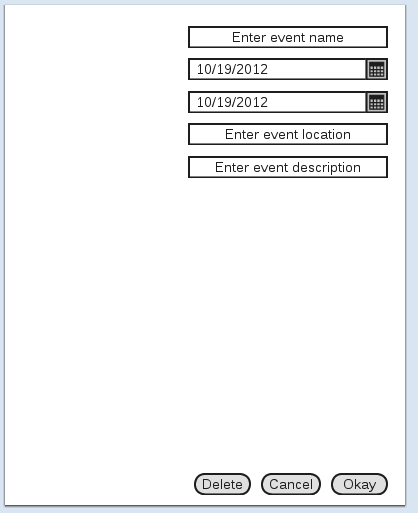
\includegraphics[scale=0.7]{CMCLGDREvent.png}
\caption{Add Event Dialog}
\label{fig:addevent}
\end{figure}

\begin{figure}[hb]
\centering
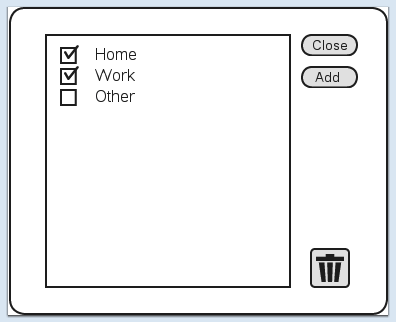
\includegraphics[scale=1]{CMCLGDRViewCalendar.png}
\caption{View Calendar Dialog}
\label{fig:viewcal}
\end{figure}

\begin{figure}[hb]
\centering
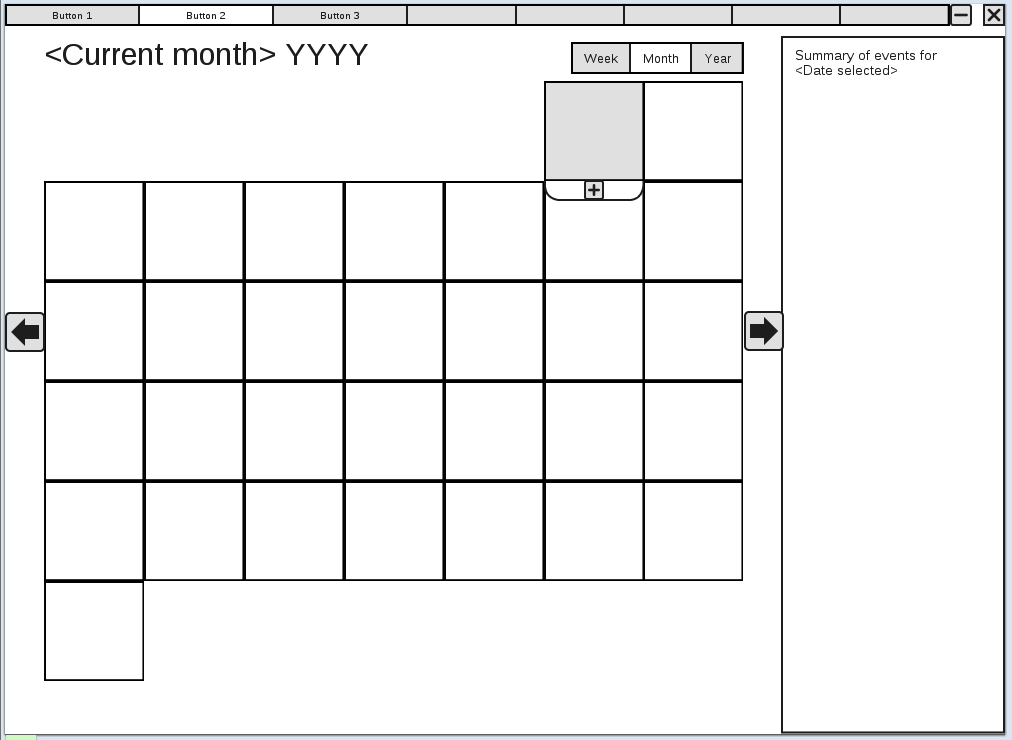
\includegraphics[scale=0.5,angle=90]{CMCLGDRMonth.png}
\caption{Month View}
\label{fig:monthview}
\end{figure}

\begin{figure}[hb]
\centering
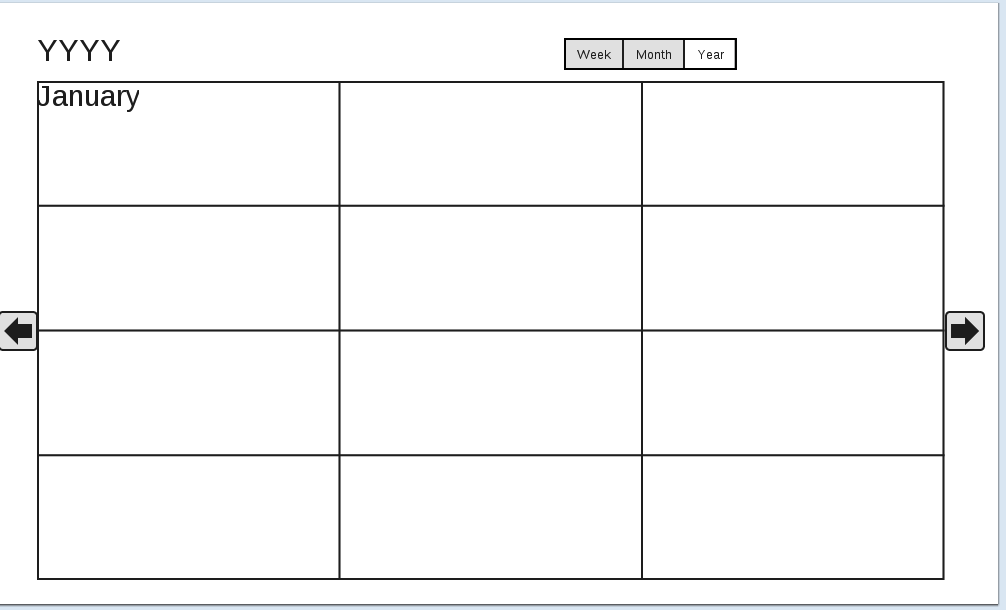
\includegraphics[scale=0.5,angle=90]{CMCLGDRYear.png}
\caption{Year View}
\label{fig:yearview}
\end{figure}

\end{document}

%%%%%%%%%%%%%%%%%%%%%%%%%%%%%%%%%%%%%%%%%%%%%%%%%%%%%%%%%%%%%%%%%%%%%%%
